\makeatletter
\cxset{author/.store in=\author@cx}
\cxset{author block=true}

\cxset{style25/.style={
 name={CHAPTER},
 numbering=arabic,
 number font-size=huge,
 number font-family=sffamily,
 number font-weight=\normalfont,
 number before=\kern0.5em,
 number position=rightname,
 chapter font-family=sffamily,
 chapter font-weight=normalfont,
 chapter font-size=huge,
 number after=\hfill\hfill\vskip1pt\hrule width\textwidth height1pt\relax\vskip1pt,
 chapter before=\hrule width\textwidth height1pt\relax\vskip1pt\hfill,
 chapter after=,
 chapter color=black!90,
 number color=black!90,
  title afterskip={\vspace{10pt}\author@cx},
 title before=\leavevmode,
 title after=\vskip1pt\hrule width\textwidth height1pt\relax,
 chapter title align=centering,
 chapter title width=.9\textwidth,
 title font-family=sffamily,
 title font-color= black!80,
 title font-weight=bfseries,
 title font-size=huge}}
\makeatother

\cxset{author=\centering\bfseries\upshape\large Yiannis Lazarides and Athena Lazarides\par\vspace{30pt}}

\cxset{style25}
\chapter{INTRODUCTION TO STYLE 25}

The interesting part of this style is that it uses roman numerals to display the counter that is in a different font than that used for the chapter name.
\lipsum*[1-2]
\begin{figure}[ht]
\centering
\fbox{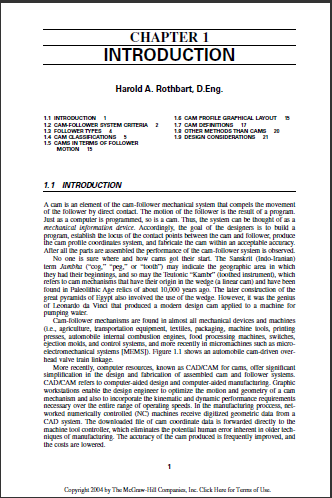
\includegraphics[width=0.5\textwidth]{./chapters/chapter25.png}}
\end{figure}

